\documentclass[a4paper, 12pt]{article}  		% classe du document

\usepackage[latin1]{inputenc} 		% packages english 
\usepackage[english]{babel}
\usepackage{url}
\usepackage{listings} 
\usepackage{color} 
\usepackage{multicol}

\definecolor{colKeys}{rgb}{0,0,1} 
\definecolor{colIdentifier}{rgb}{0,0,0} 
\definecolor{colComments}{rgb}{0,1,0} 
\definecolor{colString}{rgb}{0.6,0.1,0.1} 

\lstset{%configuration de listings 
float=hbp,% 
basicstyle=\ttfamily\small, % 
identifierstyle=\color{colIdentifier}, % 
keywordstyle=\color{colKeys}, % 
stringstyle=\color{colString}, % 
commentstyle=\color{colComments}, % 
columns=flexible, % 
tabsize=2, % 
frame=trBL, % 
frameround=tttt, % 
extendedchars=true, % 
showspaces=false, % 
showstringspaces=false, % 
numbers=left, % 
numberstyle=\tiny, % 
breaklines=true, % 
breakautoindent=true, % 
captionpos=b,% 
xrightmargin=0.8cm, % 
xleftmargin=0.8cm 
} 

%%%%%%%%%%%%%%%%%%%%%%%%%%%%%%%%%%%%%%%%%%%%%%%%%%

\usepackage[top=2.5cm, bottom=3cm, left=2.5cm, right=2.5cm]{geometry} 		% marges
\usepackage{setspace} 		% interligne

\usepackage{graphicx}  		% package figures
\usepackage{float}
\graphicspath{{images/}}

\usepackage{multirow}

\begin{document}	

\begin{titlepage}
\begin{center}
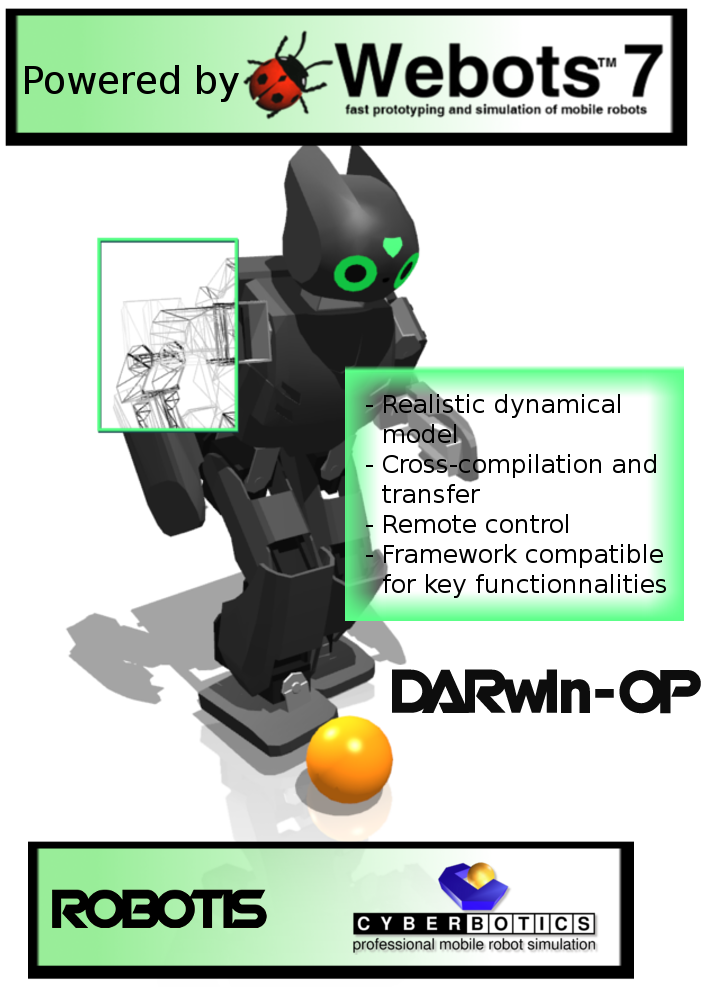
\includegraphics[width=17cm]{darwin-op.png}
\end{center}
\end{titlepage}


\begin{spacing}{0.9}
\tableofcontents
\thispagestyle{empty}
\end{spacing}
%%%%%%%%%%%%%%%%%%%%%%%%%%%%%%%%%%%%%%%%%%%%%%%%%%%%%%%%%%%%%%%%%%%%%%%%%%%%%%%%%

\newpage
\section{DARwIn-OP}
The Darwin-op is an open source miniature humanoid robot platform with advanced computational power. The name DARwIn-OP means Dynamic Anthropomorphic Robot with Intelligence-Open Platform. It is developed and manufactured by ROBOTIS (a Korean robot manufacturer) in collaboration with the University of Pennsylvania.\\

The DARwIn-OP is mainly used be university and research center for educational and research purpose. It has a total of 20 degrees of freedoms:
\begin{itemize}
\item 2 for the head.
\item 3 for each arm.
\item 6 for each leg.
\end{itemize}

This robot is very interesting because of it's low price and because it is open source (both hardware and software). For example this robot is often used for the RoboCup and even win it sometimes.\\

The DARwIn-OP robot has been fully integrated into Webots in collaboration with ROBOTIS. By using DARwIn-OP in conjunction with Webots you will have the following benefits compared to the use of ROBOTIS API directly on the real robot:
\begin{description}
\item[Simulation ] You will be able to test your controller in simulation, without any risk of damaging the robot. You will also be able to run automatically a lot of different simulations in a very small amount of time (to tune up your parameters for example), which would be impossible to do with the real robot.
\item[Cross compilation ] When your controller is fine enough in simulation, you will be able to send and run it on the real robot without changing anything to your code, just by pressing one simple button.
\item[Remote control ] To debug or understand your controller's behavior, you will be able to see in real time the state of all the sensors and actuators on the computer. This is available both in simulation and on the real robot, and here again this is done in just one click.
\item[Easy of use ] Webots greatly simplifies the programming of the robot. Indeed, Webots API is much more simple to understand and use than ROBOTIS API, moreover a very complete documentation is available for Webots.
\end{description}

%%%%%%%%%%%%%%%%%%%%%%%%%%%%%%%%%%%%%%%%%%%%%%%%%%%%%%%%%%%%%%%%%%%%%%%%%%%%%%%%%%

\newpage
\section{Simulation model}

The simulation model of DARwIn-OP has been made as close as possible to the real one. It is equiped with the following sensors and actuators :
\begin{itemize}
\item 20 servos
\item 5 LEDs (including 2 RGB ones)
\item A 3 axes accelerometer
\item A 3 axes gyroscop
\item A camera
\end{itemize}

The accelerometer return values between 0 and 1024 corresponding to values between -3 [g] to +3 [g] like on the real robot. For the gyro, it return again values between 0 and 1024, corresponding to values between -1600 [deg/sec] and +1600 [deg/sec], here again in respect of the values of the real robot. Their respective names are \textit{Accelerometer} and \textit{Gyro}.

The camera is a RGBA camera and has a basic resolution of 160x120 pixels, but it can be changed to any value. The horizontal field of view is 1.0123 [rad].\\

Concerning the LEDs, their is 2 RBG LEDs, called \textit{HeadLed} and \textit{EyeLed}, these two LEDs are each made of two separated parts, one on the head of the robots and one other small part on the back panel of the robot. There is also three other LEDs no RGB on the back panel of the robot, they are called \textit{BackLedGreen}, \textit{BackLedBlue} and \textit{BackLedRed}.\\

The name of the 20 servos are the following :

\begin{table}[H]
\begin{center}
\begin{tabular}{ | c | c | c | c | c | c | c | c |  }
\hline
ID & Name & ID & Name & ID & Name & ID & Name\\ 
\hline
\hline
1 & ShoulderR & 2 & ShoulderL & 3 & ArmUpperR & 4 & ArmUpperL \\
\hline
5 & ArmLowerR & 6 & ArmLowerL & 7 & PelvYR & 8 & PelvYL \\
\hline
9 & PelvR & 10 & PelvL & 11 & LegUpperR & 12 & LegUpperL \\
\hline
13 & LegLowerR & 14 & LegLowerL & 15 & AnkleR & 16 & AnkleL \\
\hline
17 & FootR & 18 & FootL & 19 & Neck & 20 & Head \\
\hline
\end{tabular}
%\caption{...}
\label{tab::servosName}
\end{center}
\end{table}

The corresponding position of each servos can be seen in annex \ref{sec:servopos}.\\
Each of the 20 servos have the following configuration:
\begin{table}[H]
\begin{center}
\begin{tabular}{ | c | c | c | }
\hline
maxForce & 2.5 & $N*m$ \\ 
\hline
acceleration & 55 & $rad/s^{2}$ \\ 
\hline
maxVelocity & 12.26 & $rad/s$ \\ 
\hline
dampingConstant & 0.002 & $ $ \\ 
\hline
staticFriction & 0.025 & $N*m$ \\ 
\hline
\end{tabular}
%\caption{...}
\label{tab::servosConfig}
\end{center}
\end{table}

For more information on the use of all of these sensors/actuators refer to the \textit{Reference Manual} of Webots \,\footnote{ Reference Manual available at : \url{http://www.cyberbotics.com/reference/}}.\\

The physical model is very realistic and self collision check is available. To activate the self collision expand DARwIn-OP in the scene tree and set selfCollision field to true (see figure \ref{selfCollision}). Use the self collision check only if you need it, because it is very computationally costly and can therefore significantly slow down the simulation speed.\\

\begin{figure}[H]
\begin{center}
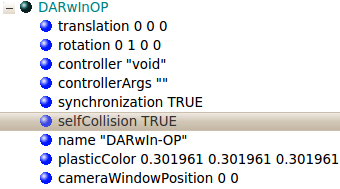
\includegraphics[width=8cm]{selfCollision.png}
\caption{Scene tree of the DARwIn-OP.}
\label{selfCollision}
\end{center}
\end{figure}

The following sensors/actuators are not present on the simulation model :
\begin{itemize}
\item The three buttons on the back of the robot are not present because they have no interest in the simulation.
\item The microphones are not present in simulation because sound is not yet supported in Webots.
\item The speakers are not present too because sound is not yet supported in Webots, but this will certainly be added soon. 
\end{itemize}

%%%%%%%%%%%%%%%%%%%%%%%%%%%%%%%%%%%%%%%%%%%%%%%%%%%%%%%%%%%%%%%%%%%%%%%%%%%%%%%%%%

\newpage
\section{Managers}

A library has been made in order to implement all the key functionalities of Robotis Framework in simulation. This library is divided in three parts called managers which implement each a module of the Framework. The first one called \textit{Gait} permits to use the walking algorithm of Robotis Framework. The second one called \textit{Motion} allows to play predefined motions stored in the file \textit{motion\_4096.bin}. The last one called \textit{Vision}, contains some image processing tools, useful for example to find a ball.\\

\subsection{Gait Manager}
This manager implement the class \textit{DARwInOPGaitManager} and allows to use the walking algorithm of the Framework.\\

A lot of parameters are available in the Framework algorithm for gait tunning. But in order to make this manager easy to use, only a subset of the parameters can be set with this manager. The other parameters are set by default on value that are known to works fine. It is however possible to change them if needed, by changing the default value that are stored in a configuration file \textit{*.ini}. In annex \ref{sec:walkParameter} all the parameters of the gait are explained. For this reasons the constructor of DARwInOPGaitManager is the following :\\

\lstset{language=c++} 
\lstset{commentstyle=\textit} 
\begin{lstlisting} 
DARwInOPGaitManager(webots::Robot *robot, const std::string &iniFilename);
\end{lstlisting}

The first parameter is the robot on which the algorithm must be applied and the second is the file name in which are stored the default parameters. The following method are available in order to modify the main parameters in your controller :\\

\lstset{language=c++} 
\lstset{commentstyle=\textit} 
\begin{lstlisting} 
void setXAmplitude(double x);
void setYAmplitude(double y);
void setAAmplitude(double a);
void setMoveAimOn(bool q);
void setBalanceEnable(bool q);
\end{lstlisting}

These are the open parameters, they have the following impact on the gait:\\
\begin{itemize}
\item X influence the length of the foot step forward, it can take any value between -1 and 1.
\item Y influence the length of the foot step in the side direction, it can take any value between -1 and 1.
\item A influence the angle of the gait and permit also to rotate during the walk, it can take any value between 0 and 1.
\item If MoveAimOn is set, it allowed to rotate around something in particular by inversing the sense of rotation, it can be very useful to turn around a ball in order to kick it in the right direction for example.
\item If BalanceEnable is set, the gyroscope is used in order to prevent the robot from falling while walking.
\end{itemize}

Finally the following method can be used in order to run the algorithm:\\
\lstset{language=c++} 
\lstset{commentstyle=\textit} 
\begin{lstlisting} 
void start();
void step(int ms);
void stop();
\end{lstlisting}
Start and stop need to be used to stop/start the algorithm and step is used to run \textit{ms} milliseconds of the algorithm.\\

It must be noticed that the gait manager need to know the position of each servos and the values of the gyro to run. It is therefore essential to enable the gyro and the position feedback of each servos before to use it, if it is not the case, a warning will appear and they will automatically be enabled.\\

\subsection{Motion Manager}
This manager implement the class \textit{DARwInOPMotionManager} and allows to play predefined motion stored in the file \textit{motion\_4096.bin}, the main motions and the corresponding id of the motion file are explained in annex \ref{sec:Motions}.\\

It is also possible to add custom motions to this file by using the tools \textit{Action Editor} \,\footnote{ More informations about this tool at : \url{www.support.robotis.com/ko/product/darwin-op/development/tools/action_editor.htm}} provided by ROBOTIS.\\

The constructor of \textit{DARwInOPMotionManager} is the following :\\
\lstset{language=c++} 
\lstset{commentstyle=\textit} 
\begin{lstlisting} 
DARwInOPMotionManager(webots::Robot *robot);
\end{lstlisting}

He only need a pointer to the robot to which it is applied. Then the following method can be used to play a motion :\\

\lstset{language=c++} 
\lstset{commentstyle=\textit} 
\begin{lstlisting} 
void playPage(int id);
\end{lstlisting}

This method only need the id of the motion that must be played.\\

\newpage
\subsection{Vision Manager}
This manager implement the class \textit{DARwInOPVisionManager}. The constructor of this class is the following :\\

\lstset{language=c++} 
\lstset{commentstyle=\textit} 
\begin{lstlisting} 
DARwInOPVisionManager(int width, int height, int hue, int hueTolerance, int minSaturation, int minValue, int minPercent, int maxPercent);
\end{lstlisting}
The parameters are the following : \\
\begin{itemize}
\item The widht of the image
\item The height of the image
\item The hue of the target to find
\item The tolerance on the hue of the target
\item The minimum saturation of the target to find
\item The minimum value of the target to find
\item The minimum percentage of target in the image to validate the result
\item The maximum percentage of target in the image to validate the result
\end{itemize}

To find the hue of your target and to understand the impact of the saturation and value you can refer to figure \ref{HSV}, for more information you can also find a lot of great documentation on internet about HSV colorspace.\\ 
\begin{figure}[H]
\begin{center}
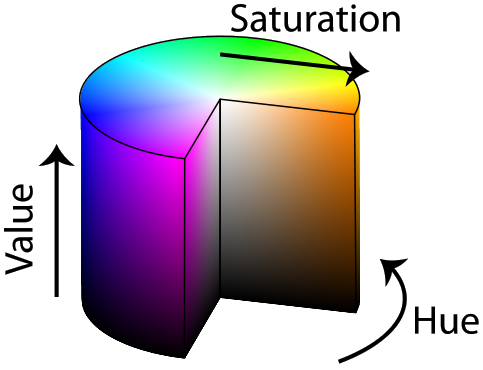
\includegraphics[width=6cm]{HSV.png}
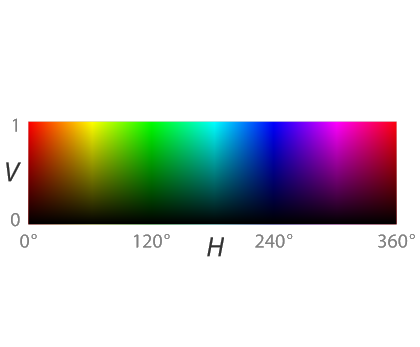
\includegraphics[width=6cm]{HV.png}
\caption{HSV colorspace}
\label{HSV}
\end{center}
\end{figure}

\newpage
When an instance of this class is created, the method \textit{getBallCenter} can be used to find the position of the target :\\

\lstset{language=c++} 
\lstset{commentstyle=\textit} 
\begin{lstlisting} 
bool getBallCenter(double &x, double &y, const unsigned char * image);
\end{lstlisting}
 
This method return true if the target has been found, and false otherwise. X and Y are references with which the result is transmitted. And image is a pointer to the image buffer. In order to find the position of the target, this method proceed to the following main steps:\\
\begin{itemize}
\item Store the BGRA version  of the image in a buffer
\item Use this buffer to convert the image to HSV format
\item Use the class \textit{Finder} of the Framework to find the target
\item Extract and save the position of the target
\end{itemize}

When this method has been called it is possible to know which pixels of the image is part of the target by using this function :\\

\lstset{language=c++} 
\lstset{commentstyle=\textit} 
\begin{lstlisting} 
bool isDetected(int x, int y);
\end{lstlisting}

This method return true if the pixel (x,y) is part of the target and false otherwise.\\


%%%%%%%%%%%%%%%%%%%%%%%%%%%%%%%%%%%%%%%%%%%%%%%%%%%%%%%%%%%%%%%%%%%%%%%%%%%%%%%%%%

\newpage
\section{Examples}

In this part we will see all the examples provided with Webots for the DARwIn-OP. We will describe how they work, how to use them and what can be done with them. All the examples can be found in WEBOTS\_HOME/projects/robots/darwin-op/worlds.\\

The following buttons are the main ones used to control the simulation (they all are situated on top of the 3D view):
\begin{table}[H]
\begin{center}
\begin{tabular}{ c l }

\includegraphics{button_open.png} & \textbf{Open world} is used to open another example. \\

\includegraphics{button_revert.png} & \textbf{Revert} is used to reload the example file and restart the simulation. \\

\includegraphics{button_play.png} & \textbf{Run} is used to start the simulation at real time speed. \\

\includegraphics{button_stop.png} & \textbf{Stop} is used to stop the simulation. \\
\end{tabular}
\end{center}
\end{table}

You will also need to use the following buttons to edit the examples (they are situated on top of the text editor):
\begin{table}[H]
\begin{center}
\begin{tabular}{ c l }

\includegraphics{button_open.png} & \textbf{Open file} is used to open a new file in the text editor. \\

\includegraphics{button_save.png} & \textbf{Save file} is used to save the current file. \\

\includegraphics{button_compile.png} & \textbf{Build} is used to build the current project. \\

\includegraphics{button_clean.png} & \textbf{Clean} is used to clean all the compilation files of the current project. \\
\end{tabular}
\end{center}
\end{table}

You can find more informations about the user interface in the corresponding chapter of the \textit{User Guide}\,\footnote{User Guide available at : \url{www.cyberbotics.com/guide}}.

\newpage
\subsection{Symmetry}

This example is very basic in order to explain the use of the servos.\\

\begin{figure}[H]
\begin{center}
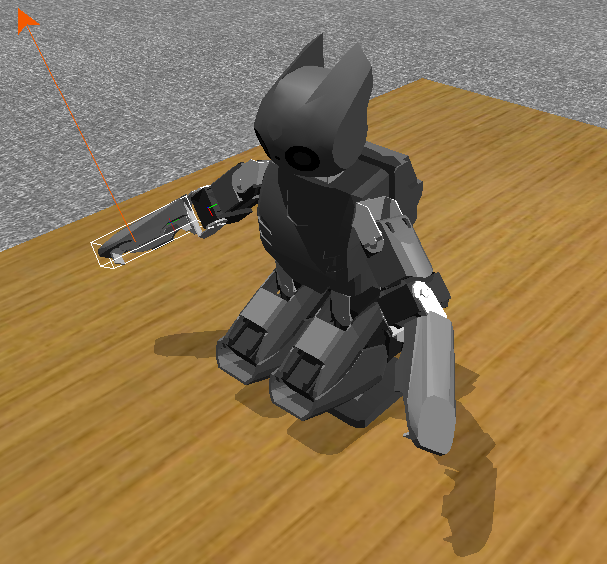
\includegraphics[width=10cm]{example_symmetry.png}
%\caption{...}
\label{example_symmetry.png}
\end{center}
\end{figure}

It start by setting the motor force of the three servos of the right arm to zero in order to completely release this arm.
Then in an infinite loop the position of the previous three servos is read and displayed.
Finally still in the loop the inverse of the position of each servos is applied on the servos of the left arm in order to mimic the motion of the right one.\\
 In order to move the right arm which is free in simulation, select the robot, then press Ctrl+Alt and left click on the arm, then without releasing the left button move the mouse. This will apply a force (symbolized by an arrow) which will make the arm to move.\\
It must be noticed that it is very important to activate the position feedback of the servos in order to read their position. In this example, this is done in the constructor.\\

You can also try to add an oscillation to the head, by adding this in your main loop:
\lstset{language=c++} 
\lstset{commentstyle=\textit} 
\begin{lstlisting} 
mServos[18]->setPosition(sin(getTime()));
\end{lstlisting}

Then save the file, press the build button and finally revert the simulation to start the new controller.\\

This example is well suited for the cross-compilation and we recommended that you start by testing the cross-compilation tool by using this example.\\

\newpage
\subsection{VisualTracking}

This example illustrate the use of the camera (including the vision manager) and of the RGB LEDs.\\

\begin{figure}[H]
\begin{center}
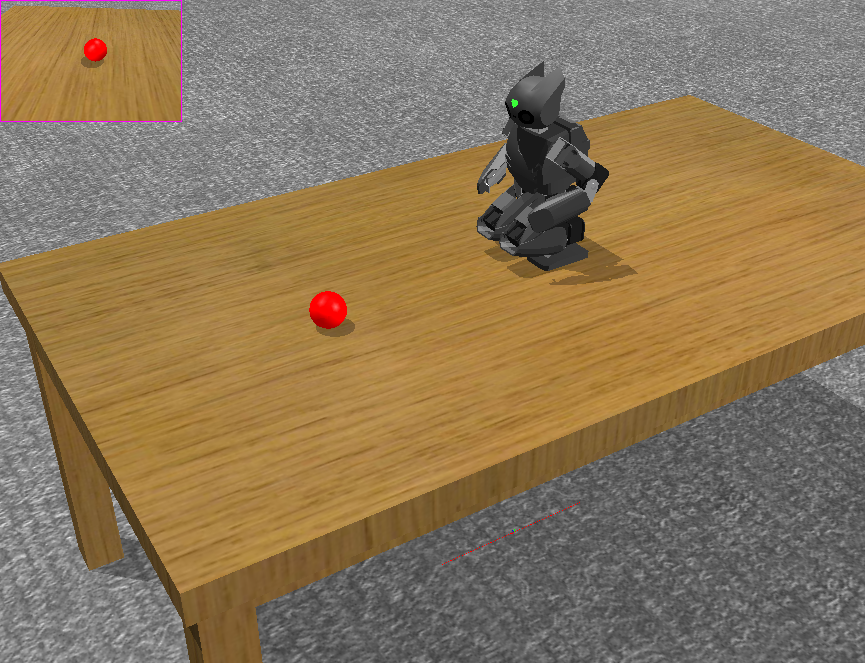
\includegraphics[width=10cm]{example_visualTracking.png}
%\caption{...}
\label{example_visualTracking.png}
\end{center}
\end{figure}

In the infinite loop the vision manager is used to find the red ball. 
Then if the ball has been found the head led is set to green and otherwise to red.
Then again if the ball has been found the position of the two servos of the head is corrected to watch in the direction of the ball. To move the ball in simulation, press Ctrl+Shift and move the ball with the left button of the mouse pressed on it.\\

Try to change the color of the LED by changing this line :
\lstset{language=c++} 
\lstset{commentstyle=\textit} 
\begin{lstlisting} 
mHeadLED->set(0xFF0000);
\end{lstlisting}
Here the color is set in hexadecimal. The format is R8G8B8: The most significant 8 bits (left hand side) indicate the red level (between 0x00 and 0xFF). Bits 8 to 15 indicate the green level and the least significant 8 bits (right hand side) indicate the blue level. For example, 0xFF0000 is red, 0x00FF00 is green, 0x0000FF is blue, 0xFFFF00 is yellow, etc.\\

Try also to use the other RGB LED, this is done simply be exchanging \textit{mHeadLED} by \textit{mEyeLED}.\\

Here again this example is well suited for cross-compilation. You can adjust the color of the ball by changing the value in the constructor of DARwInOPVisionManager if your ball is of another color.\\


\newpage
\subsection{Walk}

This example illustrate the use of the gait and motion manager, the use of the keyboard, and also the use of the accelerometer.\\

\begin{figure}[H]
\begin{center}
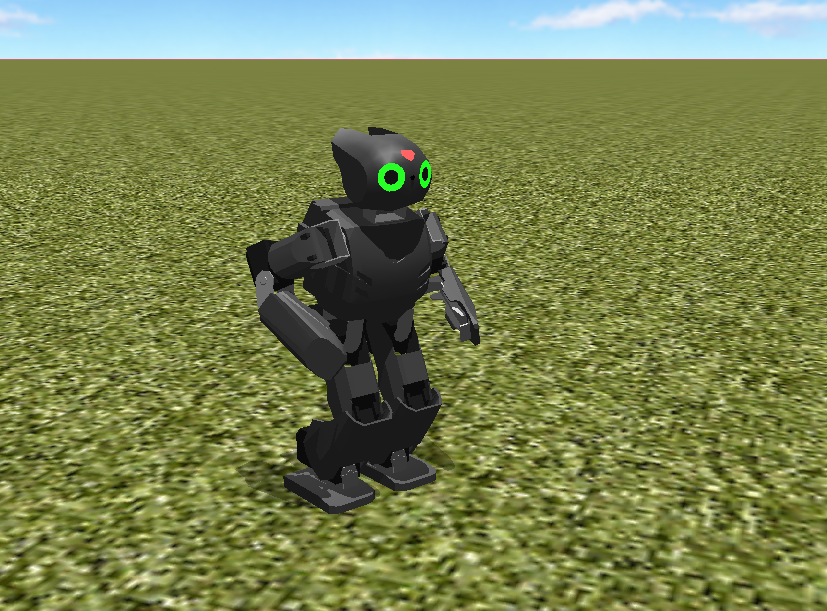
\includegraphics[width=10cm]{example_walk.png}
%\caption{...}
\label{example_walk.png}
\end{center}
\end{figure}

At the beginning of the controller, the motion manager is used to make the robot stand up, then the controller enter an infinite loop.
The first things done in the loop is to check if the robot has not fallen, this is done by using the accelerometer. Then if the robot has fallen, the motion manager is used in order to make the robot to stand up. 
Then the keyboard is read, if the key \textit{Page Up} is pressed it make the robot start to walk, contrary if key \textit{Page Down} is pressed the robot stop to walk.
Then the keys up/down/right/left are used to make the robot turn and move forward/backward, severals key can be used in the same time.\\

Try to add some more action by using more key. You can for example use the keys \textit{KEYBOARD\_NUMPAD\_LEFT} and \textit{KEYBOARD\_NUMPAD\_RIGHT} to make a left/right shoot (page 13 and 12 in motion manager).\\

You can also use another key to make the robot walk quicker or slower (change the XAmplitude sent to the gait manager, value accepted must be between -1 and 1).\\

This example work in cross-compilation but you will need to connect an usb keyboard to the robot. It is recommended to test this example with remote control in order to use the computer's keyboard instead.\\


\newpage
\subsection{Soccer}

This is a very complete example which used the three managers and almost all of the sensors.\\

\begin{figure}[H]
\begin{center}
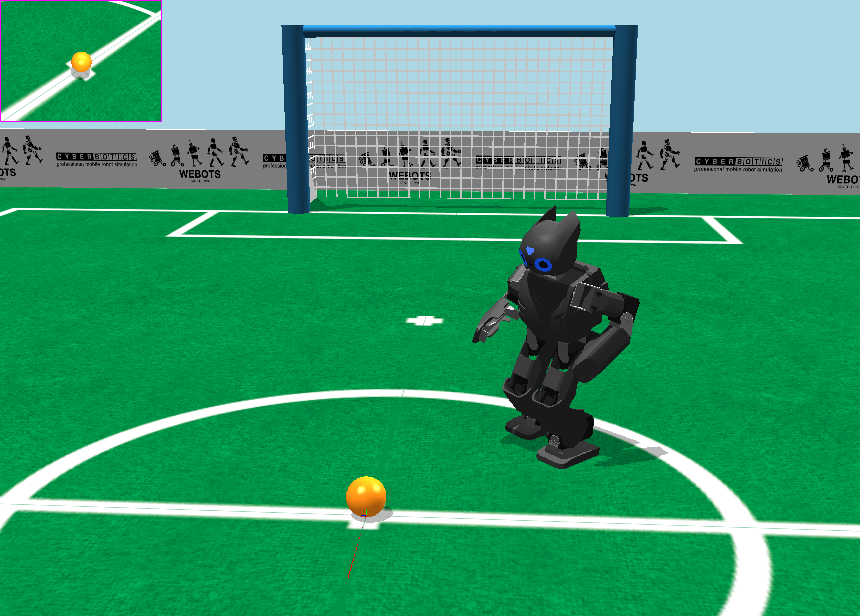
\includegraphics[width=10cm]{example_sample.png}
%\caption{...}
\label{example_sample.png}
\end{center}
\end{figure}

The controller is a very simple soccer player. It used most of the tools used in the previous example. We recommend you to study it by yourself and of course to improve it.\\

To extend your controller you can add new files to the project, but do not forget to also add them to the makefile (add the cpp files to the \textit{CXX\_SOURCES} section).\\

This example work in cross-compilation. But we recommend you to test it on a soft ground and away from any source of danger (stairs, hot surface ...), because the robot will move a lot and it is not excluded that it fall sometimes.\\


%%%%%%%%%%%%%%%%%%%%%%%%%%%%%%%%%%%%%%%%%%%%%%%%%%%%%%%%%%%%%%%%%%%%%%%%%%%%%%%%%

\newpage
\section{Robot Window}

When double clicking on the robot, a new window appears. This window is called \textit{Robot Window}, it has severals tabs who permits to do a lot of different things. The first four tabs concerns only the simulation and they will be describe here, the last tab is used to interact with the real robot and will therefore be describe in the next sections.\\

In the case PEU probable of something going wrong with the \textit{Robot Window} (freeze, bad behavior, ...) you can at any time restart it by pressing the revert button of the simulation.\\

\paragraph*{Accelerometers} 
This tab can be used to investigate the values of the accelerometer while the controller is running. If the checkbox is checked, the values of the accelerometer are shown and plotted on the graph in real time. Four different types of graph can be plot. The first three are one axis in function of an other, and the last one, plot the value of the three axes in function of the time. The corresponding colors are the following :\\
\begin{itemize}
\item Red for axis X
\item Green for axis Y
\item Blue for axis Z
\end{itemize}

\begin{figure}[H]
\begin{center}
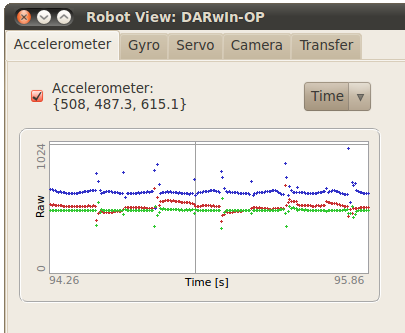
\includegraphics[width=10cm]{window_accel.png}
\label{window_accel}
\end{center}
\end{figure}

You can at any time click on the graph to adjust the scale to the data currently plotted.\\

\newpage
\paragraph*{Cameras}
This tab is very simple, if the checkbox is checked, the picture of the camera is shown and updated in real time.\\

\begin{figure}[H]
\begin{center}
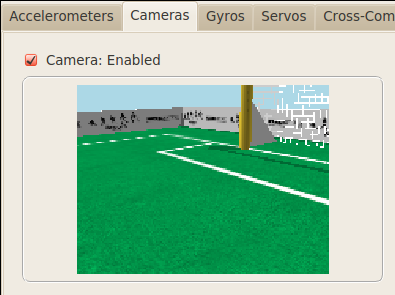
\includegraphics[width=10cm]{window_camera.png}
\label{window_camera}
\end{center}
\end{figure}

\paragraph*{Gyro}
This tab is very similar to the accelerometer tab but for the gyro. If the checkbox is checked, the values of the gyro are shown and plotted on the graph in real time. Here again the four different types of graph can be plot. \\

\begin{figure}[H]
\begin{center}
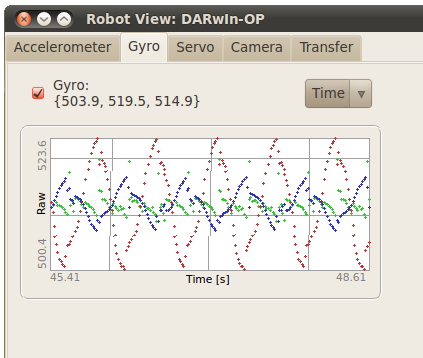
\includegraphics[width=10cm]{window_gyro.png}
\label{window_gyro}
\end{center}
\end{figure}

\newpage
\paragraph*{Servos}
Finally this last tab can be used to see and influence the state of each servos. The use of each servos in the robot window can separately be set by checking/unchecking the corresponding checkbox of the servos. If the checkbox is checked, the value of the servo is shown and plotted in function of the time. On the graph, two different colors are used to distinguish the target value (in red) and the real value (in black). It is also possible to manually change the value of the servo by using the slider beside the graph.\\

\begin{figure}[H]
\begin{center}
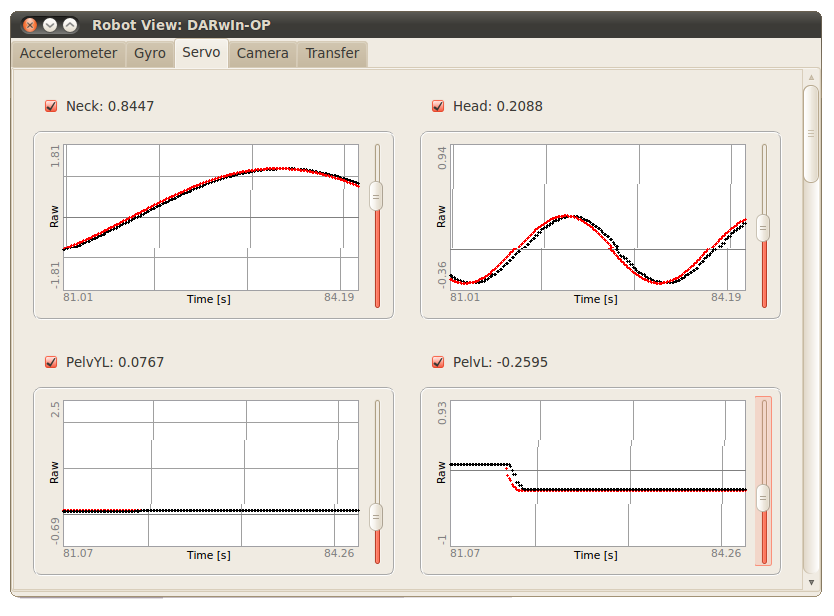
\includegraphics[width=14cm]{window_servos.png}
\label{window_servos}
\end{center}
\end{figure}


%%%%%%%%%%%%%%%%%%%%%%%%%%%%%%%%%%%%%%%%%%%%%%%%%%%%%%%%%%%%%%%%%%%%%%%%%%%%%%%%%

\newpage
\section{Cross-compilation}

To send your controller to the real robot and make it run on it, go the tab \textit{Transfer} of the robot window (figure \ref{window_cross}).

\begin{figure}[H]
\begin{center}
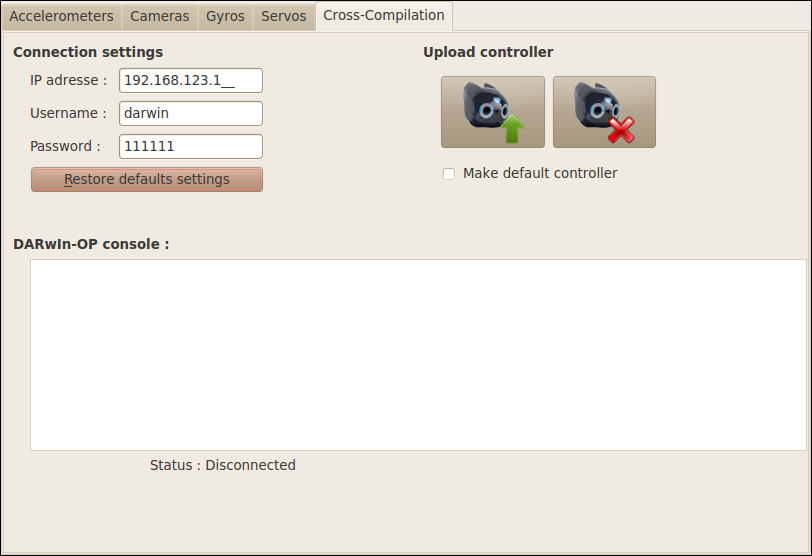
\includegraphics[width=13cm]{window_cross.png}
\caption{Tab Transfer of the robot window.}
\label{window_cross}
\end{center}
\end{figure}

The first thing to do is to set the connections settings. The first setting is the IP address of the robot. If you use an ethernet cable to connect to the robot, the IP address is 192.168.123.1. But if you use a wifi connection with the robot the address is not fixed, to know it execute the command \textit{ifconfig} on the robot, the IP address is the \textit{inet addr} of wlan0 (warning, the adress can sometimes change without any specific reasons). The second parameters is the username with which you log-on on the robot, if you do not have explicitly changed it, the username is \textit{darwin}. Finally the last parameters is the password corresponding to the username, here again, if you do not have explicitly changed it, the password is \textit{111111}. Each time you connect successfully to the robot, all the settings are saved in order that it is not necessary to set them each time you start the program. If you want to restore the default parameters of the connection, just click on the button \textit{Restore default settings} (Alt+r).\\

Before you can send your controller to the real robot you have to change the file Makefile.darwin-op to suit to your project. If you have added new file to the project, do not forget to add them to the \textit{CXX\_SOURCES} and if you have changed the project name change also the \textit{TARGET}.\\

\newpage
Before to send the controller you will also need to complete the \textit{Robot Config} section of the file \textit{config.ini}. You have two parameters to complete :
\begin{description}
\item[Time step] The time step in milliseconds must be specified in the field \textit{time\_step}, a minimal time step of 16ms is requested, if no time step (or a time step smaller than 16ms) is set, the default time step of 16ms is set. Warning : Depending on the complexity of you controller, a time step of 16ms can not always be respected. For example using the camera or the manager can slow done the speed, so enable them only if you really need them.\\
\item[Camera resolution] The horizontal and vertical resolution of the camera must be set in the fields \textit{camera\_width} and \textit{camera\_height}. Only the resolutions specified in table \ref{tab:cameraResolution} are supported, if another resolution is set, the default resolution of 320x240 will be used.\\
\end{description}

\begin{table}[H]
\begin{center}
\begin{tabular}{ | c | c | c | }

\hline
Width [pixel] & Height [pixel] & FPS \\ 
\hline
\hline
320 & 240 & 30 \\
\hline
640 & 360 & 30 \\
\hline
640 & 400 & 30 \\
\hline
640 & 480 & 30 \\
\hline
768 & 480 & 28 \\
\hline
800 & 600 & 22.5 \\
\hline
\end{tabular}
\caption{Camera resolutions supported by the camera of the DARwIn-OP.}
\label{tab:cameraResolution}
\end{center}
\end{table}

\subsection{Send a controller to the robot}
To test your controller on the real robot press the following button :
\begin{figure}[H]
\begin{center}

\includegraphics[width=2.5cm]{send.png}
\label{send}
\end{center}
\end{figure}

Webots will then connect to the robot, if any error appear during the connection, the reason will be shown. If it is the first time you connect the robot with Webots, Webots will install all the files needed on the robot. This can take some times and some step are longer than other, so be patient please, this is only on the first connection, the next ones will be shorter. You can also see in real time what is appening in the \textit{DARwIn-OP console}. Webots will also stop the auto start of the demo program at the startup of the robot, but don't worry the program is not suppressed and the auto start can easily be reinstalled (explanation follows).\\


Then the controller code itself is send to the robot. All the directory of the controller is send to the robot, so please put all the files needed by your controller in the same directory. The controller itself is then compiled for the robot and you can see the compilation in the \textit{DARwIn-OP console}. If the compilation success and the robot is close to the start position (figure \ref{start_position}) the controller will be initialized (head and eyes LED in red) and then started (head and eyes LED in green).\\

\begin{figure}[H]
\begin{center}
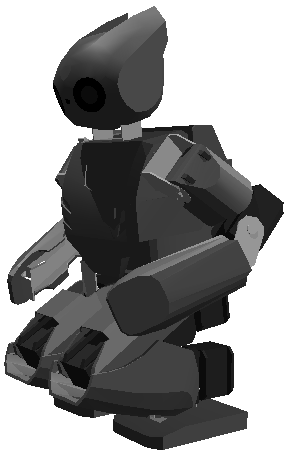
\includegraphics[width=5cm]{start_position.png}
\label{start_position}
\caption{Start position of the robot. The robot is sit down (same start position that in simulation).}
\end{center}
\end{figure}

It is recommended when testing a new controller whose behavior is not very certain to hold the robot by its handle.\\

To stop the controller press the following button :
\begin{figure}[H]
\begin{center}

\includegraphics[width=2.5cm]{stop.png}
\label{stop}
\end{center}
\end{figure}

This will stop the controller and clean all files previously sent to the robot.\\

You can also stop the controller by pressing the right button at the back of the robot. This will not entirely stop the controller but will at least avoid the robot from moving. It will also release the torque of all the servos.\\

\subsection{Permanently install a controller to the robot}
If you want to install the controller on the real robot, check the checkbox \textit{Make default controller}. Then when you press the button to send the controller to the real robot, instead of running after the compilation, the controller is set to start automatically at the startup of the robot without any need of Webots or any computer. But warning the robot still need to be in the start position when starting but their wont be any verification on the position, it is your responsibility to make sure that you always start the robot in this position (starting from an unknown position is not safe).\\

\subsection{Uninstall Webots from the robot}
If you plain to not use anymore Webots with your DARwIn-OP, you can uninstall all the files installed on the DARwIn-OP by Webots by pressing this button :
\begin{figure}[H]
\begin{center}

\includegraphics[width=2.5cm]{uninstall.png}
\label{uninstall}
\end{center}
\end{figure}

This will restore your robot like it was before installing Webots files to it. Even the demo program will again automatically start at the startup of the robot. But if you send again a controller to the robot with Webots, all the files will again be installed. You can also use this button to reinstall all Webots files to the robot if you think something went wrong during the installation.\\ 

If you install a new version of Webots on your computer the Webots files on the robot will automatically been update at the sending of the first controller (don't worry if you use severals version of Webots, an older version can not erase files from a newer version).\\

\subsection{Dynamixel MX28 firmware}
The cross-compilation has been optimized for the lasts firmware versions of the servos. You need to have at least version 27 of the firmware installed on all the servos, if this is not the case (on old DARwIn-OP robot for example) you will be informed when you will try to send a controller to the real robot. In order to update the firmware version please use the tool \textit{Firmware Installer}\,\footnote{ More informations about this tool at : \url{www.support.robotis.com/ko/product/darwin-op/development/tools/firmware_installer.htm}} from ROBOTIS.\\

\newpage
\subsection{Using speaker}
As speaker are not present in Webots, it is not possible to use the speakers in simulation. In cross-compilation it is still possible to play sound by using this two function :\\
\lstset{language=c++} 
\lstset{commentstyle=\textit} 
\begin{lstlisting} 
virtual void playFile(const char* filename);
virtual void playFileWait(const char* filename);
\end{lstlisting}
Filename is the path to an audio file (MP3 for example). The function \textit{playFile} play the file without stopping the controller while the function \textit{playFileWait} stop the controller as long as the audio file is not finished.\\

In order to use them you have to use something similar to this :\\
\lstset{language=c++} 
\lstset{commentstyle=\textit} 
\begin{lstlisting} 
mSpeaker = getSpeaker("Speaker");
mSpeaker->enable(mTimeStep);
mSpeaker->playFile("hello.mp3"); // the file is in the same directory that the controller
\end{lstlisting}

And do not forget to include \textit{webots/Speaker.hpp}.\\

Because Speaker are not yet present in simulation we recommend you to put all your code concerning the speaker in a \textit{\#ifdef CROSSCOMPILATION} in order to keep the same code running in simulation and on the real robot. Here is an example :\\
\lstset{language=c++} 
\lstset{commentstyle=\textit} 
\begin{lstlisting} 
#ifdef CROSSCOMPILATION
  mSpeaker = getSpeaker("Speaker");
  mSpeaker->enable(mTimeStep);
#endif
\end{lstlisting}

Severals audio files are already present on the robot in the folder \textit{/darwin/Data/mp3/}, you can freely use them like this :\\
\lstset{language=c++} 
\lstset{commentstyle=\textit} 
\begin{lstlisting} 
mSpeaker->playFile("/darwin/Data/mp3/FileName.mp3"); // this file is already on the robot, no need to send it.
\end{lstlisting}

The annex \ref{sec:audioFile} reference all the audio files available.\\

%%%%%%%%%%%%%%%%%%%%%%%%%%%%%%%%%%%%%%%%%%%%%%%%%%%%%%%%%%%%%%%%%%%%%%%%%%%%%%%%%

\newpage
\section{Remote control}



%%%%%%%%%%%%%%%%%%%%%%%%%%%%%%%%%%%%%%%%%%%%%%%%%%%%%%%%%%%%%%%%%%%%%%%%%%%%%%%%%

\appendix
\newpage
\pagenumbering{Roman} %switch to roman enumeration

%%%%%%%%%%%%%%%%%%%%%%%%%%%%%%%%%%%%%%%%%%%%%%%%%%%%%%%%%%%%%%%%%%%%%%%%%%%%%%%%%

\section{Walking parameters} \label{sec:walkParameter}

This annex explain all the parameters that can be set in the configuration file (.ini) to tune the gait.\\ 

\paragraph*{X offset}
is the offset of the feet in the direction X. Unit is in millimeter.
\begin{figure}[H]
\begin{center}
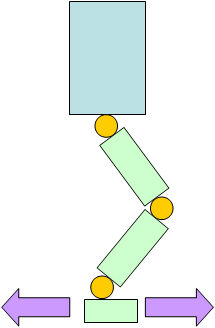
\includegraphics[width=3cm]{x_offset.jpg}
\caption{Walking : x offset parameters}
\label{x_offset}
\end{center}
\end{figure}

\paragraph*{Y offset}
is the offset of the feet in the direction Y. Unit is in millimeter.
\begin{figure}[H]
\begin{center}
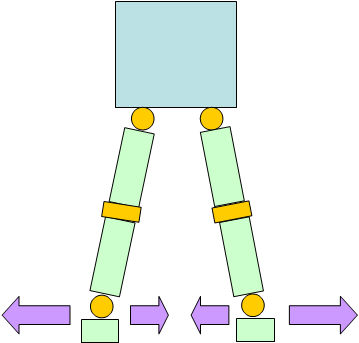
\includegraphics[height=6cm]{y_offset.jpg}
\caption{Walking : y offset parameters}
\label{y_offset}
\end{center}
\end{figure}

\newpage
\paragraph*{Z offset}
is the offset of the feet in the direction Z. Unit is in millimeter.
\begin{figure}[H]
\begin{center}
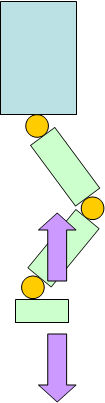
\includegraphics[height=6cm]{z_offset.jpg}
\caption{Walking : z offset parameters}
\label{z_offset}
\end{center}
\end{figure}

\paragraph*{Roll offset}
is the angle offset at the feet along X axis. Unit is in degree.
\begin{figure}[H]
\begin{center}
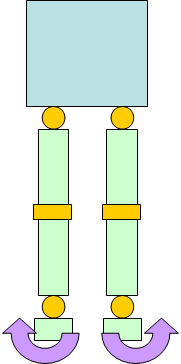
\includegraphics[height=6cm]{roll_offset.jpg}
\caption{Walking : roll offset parameters}
\label{roll_offset}
\end{center}
\end{figure}

\newpage
\paragraph*{Pitch offset}
is the angle offset at the feet along Y axis. Unit is in degree.
\begin{figure}[H]
\begin{center}
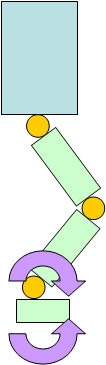
\includegraphics[height=6cm]{pitch_offset.jpg}
\caption{Walking : pitch offset parameters}
\label{pitch_offset}
\end{center}
\end{figure}

\paragraph*{Yaw offset}
is the angle offset of the leg along Z axis. Unit is in degree.
\begin{figure}[H]
\begin{center}
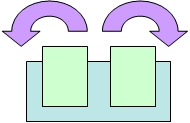
\includegraphics[height=2.5cm]{yaw_offset.jpg}
\caption{Walking : yaw offset parameters}
\label{yaw_offset}
\end{center}
\end{figure}

\paragraph*{Hip pitch offset}
is the tilt of DARwIn-OP's body. It uses a special unit of the motor correspondig to 2.85 degree.
\begin{figure}[H]
\begin{center}
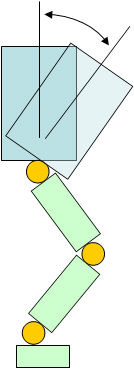
\includegraphics[height=6cm]{hip_pitch_offset.jpg}
\caption{Walking : hip pitch offset parameters}
\label{hip_pitch_offset}
\end{center}
\end{figure}

\newpage
\paragraph*{Period time}
is the time required for DArwIn-Op to complete two full steps (left and right foot). Unit is in millisecond.
\begin{figure}[H]
\begin{center}
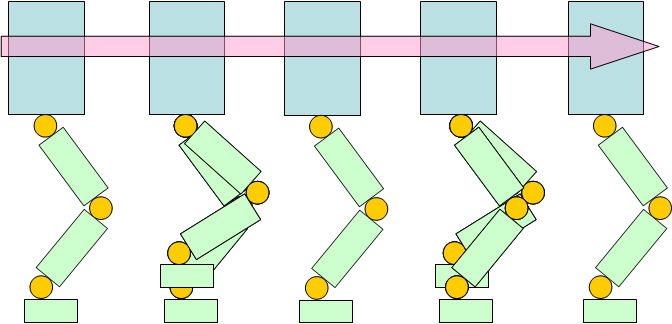
\includegraphics[width=8cm]{period_time.jpg}
\caption{Walking : period time parameters}
\label{period_time}
\end{center}
\end{figure}

\paragraph*{DSP ratio}
is the ratio between the time when both feet are on the ground to only one foot (either left or right) is on the ground.
\begin{figure}[H]
\begin{center}
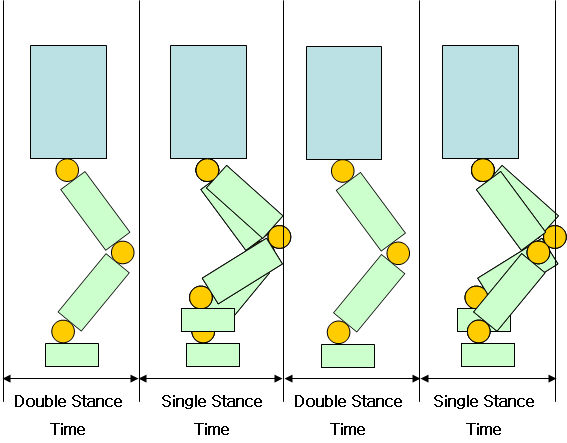
\includegraphics[width=8cm, height=5.5cm]{dsp_ratio.jpg}
\caption{Walking : dsp ratio parameters}
\label{dsp_ratio}
\end{center}
\end{figure}

\newpage
\paragraph*{Step forward back ratio}
is the differential distance according to X direction, between DARwIn-OP's left and right foot during walk. Unit is in millimeter.
\begin{figure}[H]
\begin{center}
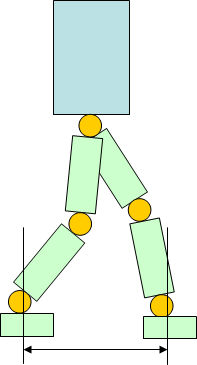
\includegraphics[height=4.5cm]{step_forward_back_ratio.jpg}
\caption{Walking : step forward back ratio parameters}
\label{step_forward_back_ratio}
\end{center}
\end{figure}

\paragraph*{Foot height}
is the maximum height of the foot during the step. Unit is in millimeter.
\begin{figure}[H]
\begin{center}
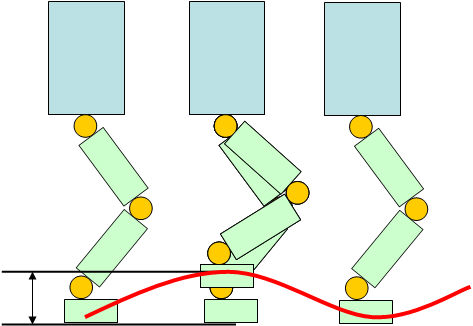
\includegraphics[height=4.5cm]{foot_height.jpg}
\caption{Walking : foot height parameters}
\label{foot_height}
\end{center}
\end{figure}

\paragraph*{Swing right left}
is the left and right Swaying of DARwIn-OP's body during walking. Unit is in millimeter.
\begin{figure}[H]
\begin{center}
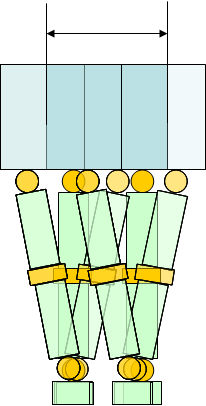
\includegraphics[height=6cm]{swing_right_left.jpg}
\caption{Walking : swing right left parameters}
\label{swing_right_left}
\end{center}
\end{figure}

\paragraph*{Swing top down}
is the up and down swaying of DARwIn-OP's body during walking. Unit is in millimeter.
\begin{figure}[H]
\begin{center}
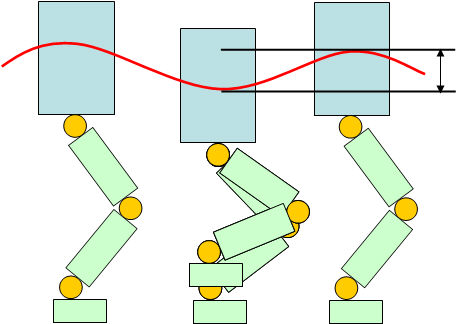
\includegraphics[height=5cm, width=8.5cm]{swing_top_down.jpg}
\caption{Walking : swing top down parameters}
\label{swing_top_down}
\end{center}
\end{figure}

\paragraph*{Pelvis offset}
is angle offset at the pelvis along X axis. It uses a special unit of the motor correspondig to 2.85 degree.
\begin{figure}[H]
\begin{center}
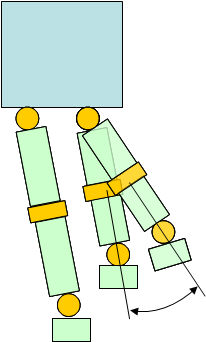
\includegraphics[height=5cm, width=3.7cm]{pelvis_offset.jpg}
\caption{Walking : pelvis offset parameters}
\label{pelvis_offset}
\end{center}
\end{figure}

\paragraph*{Arm swing gain}
is the gain that influence the movements of the arm during walking.

\paragraph*{Balance knee gain}
is the gain at the knee level for the front/back balance

\paragraph*{Balance ankle pitch gain}
is the gain at the ankle level for the front/back balance.

\paragraph*{Balance hip roll gain}
is the gain at the hip level for the lateral balance. Since lateral balance do not work very well in simulation, we recommend you tu put this parameters to 0.

\paragraph*{Balance ankle roll gain}
is the gain at the ankle level for the lateral balance. Since lateral balance do not work very well in simulation, we recommend you tu put this parameters to 0.


%%%%%%%%%%%%%%%%%%%%%%%%%%%%%%%%%%%%%%%%%%%%%%%%%%%%%%%%%%%%%%%%%%%%%%%%%%%%%%%%%

\section{Motions files} \label{sec:Motions}

\begin{table}[H]
\begin{center}
\begin{tabular}{ | c | c | c | c | }

\hline
ID & Name & Description & Recommended initial position \\ 
\hline
\hline
1 & ini & Move to standing position & Standing up \\
\hline
2 & OK & Nods head & Standing up \\
\hline
3 & no & Shakes head & Standing up \\
\hline
4 & hi & Tilts forward & Standing up \\
\hline
6 & talk1 & Holds out his hand & Standing up \\
\hline
9 & walkready & Prepares to walk & Standing up \\
\hline
10 & f up & Gets up & Lying face against the ground \\
\hline
11 & b up & Gets up & Lying back on the ground \\
\hline
12 & rk & Right shoot & Standing up \\
\hline
13 & lk & Left shoot & Standing up \\
\hline
15 & sit down & Sits & Standing up \\
\hline
16 & stand up & Stands up & Seated \\
\hline
17 & mul1 & Gets balanced on the head & Standing up \\
\hline
23 & d1 & Does yes with the arm & Standing up \\
\hline
24 & d2 & Applaud & Standing up \\
\hline
27 & d3 & Does yes with the arm and head & Standing up \\
\hline
29 & talk2 & Holds out his hand & Standing up \\
\hline
31 & d4 & Stretches in front and rear & Standing up \\
\hline
38 & d2 & Wave with the hand & Standing up \\
\hline
41 & talk2 & Presents himself & Standing up \\
\hline
54 & int & Applaud louder & Standing up \\
\hline
57 & int & Applaud & Standing up \\
\hline
70 & rPASS & Performs a pass with the right foot & Standing up \\
\hline
71 & lPASS & Performs a pass with the left foot & Standing up \\
\hline
90 & lie down & Lies on the front & Standing up \\
\hline
91 & lie up & Lies on the back & Standing up \\
\hline
237 & sitdown & Jumps up and down & Standing up \\
\hline
239 & sitdown & Jumps up and down quickly & Standing up \\
\hline
\end{tabular}
\caption{Motions stored in the motions files.}
\label{tab::Motions}
\end{center}
\end{table}

%%%%%%%%%%%%%%%%%%%%%%%%%%%%%%%%%%%%%%%%%%%%%%%%%%%%%%%%%%%%%%%%%%%%%%%%%%%%%%%%%

\section{Audio files available} \label{sec:audioFile}

\begin{table}[H]
\begin{center}
\begin{tabular}{ | c | c | c |  }

\hline
File & Lenght [sec] & Size [kB] \\ 
\hline
\hline
Autonomous soccer mode.mp3 & 1 & 29 \\
\hline
Bye bye.mp3 & 1 & 18.4 \\
\hline
Clap please.mp3 & 1 & 20.4 \\
\hline
Demonstration ready mode.mp3 & 2 & 31.5 \\
\hline
Headstand.mp3 & 1 & 19.2 \\
\hline
Interactive motion mode.mp3 & 1 & 29.8 \\
\hline
Introduction.mp3 & 16 & 258.8 \\
\hline
Left kick.mp3 & 1 & 17.2 \\
\hline
No.mp3 & 1 & 13.5 \\
\hline
Oops.mp3 & 1 & 14.7 \\
\hline
Right kick.mp3 & 1 & 18.4 \\
\hline
Sensor calibration complete.mp3 & 2 & 36.4 \\
\hline
Sensor calibration fail.mp3 & 2 & 37.2 \\
\hline
Shoot.mp3 & 1 & 15.5 \\
\hline
Sit down.mp3 & 1 & 20.4 \\
\hline
Stand up.mp3 & 1 & 19.6 \\
\hline
Start motion demonstration.mp3 & 2 & 34.3 \\
\hline
Start soccer demonstration.mp3 & 2 & 34.3 \\
\hline
Start vision processing demonstration.mp3 & 2 & 42.9 \\
\hline
System shutdown.mp3 & 1 & 26.2 \\
\hline
Thank you.mp3 & 1 & 17.2 \\
\hline
Vision processing mode.mp3 & 1 & 28.2 \\
\hline
Wow.mp3 & 1 & 17.6 \\
\hline
Yes.mp3 & 1 & 16.8 \\
\hline
Yes go.mp3 & 1 & 24.1 \\
\hline
\end{tabular}
\caption{Audio files already available on the robot in the directory /darwin/Data/mp3/}
\label{tab::audioFile}
\end{center}
\end{table}

%%%%%%%%%%%%%%%%%%%%%%%%%%%%%%%%%%%%%%%%%%%%%%%%%%%%%%%%%%%%%%%%%%%%%%%%%%%%%%%%%

\section{Position of each servos} \label{sec:servopos}
\vspace{5cm}

\begin{figure}[H]
\begin{center}
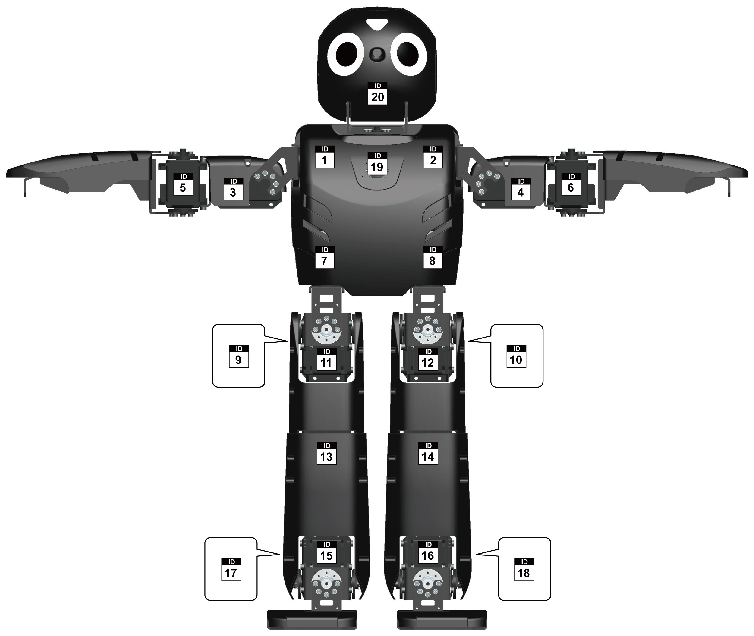
\includegraphics[width=16cm]{DARwIn-OP_Actuator.png}
\label{Actuator}
\end{center}
\end{figure}


%%%%%%%%%%%%%%%%%%%%%%%%%%%%%%%%%%%%%%%%%%%%%%%%%%%%%%%%%%%%%%%%%%%%%%%%%%%%%%%%%

\end{document}
